\section{Introduction}\label{intro}
\subsection{Basics of Nuclear Magnetic Resonance}\label{basics}
Nuclear Magnetic Resonance, or short NMR, can only be observed for molecules with a non-zero magnetic dipole moment. For a given nuclei, whose spin $\vec{J}$ is unequal to 0, one can calculate its magnetic dipole moment as
\begin{equation}
	\label{1}
	\vec{\mu} = \hbar \gamma \vec{J}.
\end{equation}
Where $\gamma$ is the gyromagnetic factor. In this experiment we will look at exclusively protons, which have $\gamma_{proton} = 2.6752 \cdot 10^8 sec^{-1} Tesla^{-1}$.
\vspace{3mm} \\
The magnetization of $N$ nuclei can be obtained, by summing over all nuclei per unit volume
\begin{equation}
	\label{2}
	\vec{M} = \dfrac{1}{V} \sum^{N}_{i=1} \vec{\mu_i}
\end{equation}
With the assumption of a weak field $(\mu B << kT)$, which is the case in our experiment, one can approximate $\vec{M} \sim \frac{\vec{B_{0}}}{T}$ according to Curie's Law. 
\vspace{5mm} \\
In general, the magnetization can have an arbitrary direction relative to the external field. In the following we will decompose it into the components $\vec{M_{\parallel}}$ (anti-)parallel and $\vec{M_{\perp}}$ perpendicular to the external field. 
The magnetic dipole interacts with the $\vec{B_{0}}$ and as a result the general state of magnetization will dissipate it's excitation energy and reach the ground state, i.e. $\vec{M_{\parallel}}$, asymptotically on a characteristic time scale. The dissipated energy can be expressed by
\begin{equation}
	\label{5}
	\Delta E = - \vec{\mu} \cdot \vec{B_0}
\end{equation}
\vspace{3mm} \\
This interaction results in a torque and since $\vec{B_{0}}$ is parallel to $\vec{M_{\parallel}}$, the torque only acts on $\vec{M_{\perp}}$.
\begin{equation}
	\label{6}
	\vec{\tau} = \vec{M} \times \vec{B_{0}}
\end{equation}
Without a relaxation processes, the rate of change is given by
\begin{equation}
	\label{7}
	\dfrac{d\vec{M_{\perp}}}{dt} = - \gamma \vec{M_{\perp}} \times \vec{B_{0}}.
\end{equation}
This differential equation can be solved by an Ansatz $\vec{M} = M_{\parallel}(cos(\omega_{L} t),sin(\omega_{L} t),0)$ with $\omega_{L}$ being the Larmor frequency 
\begin{equation}
	\label{8}
	\omega_{L} = \gamma B_{0}
\end{equation}
Let's consider the ground state magnetization $\vec{M}$, which is parallel to $\vec{B_0}$ and the z-axis. If we apply a sinusoidal voltage with frequency $\omega_{HF}$ to a coil which is coiled along the x-axis, it will result in a solenoidal magnetic field $\vec{B_1}$ which is perpendicular to $\vec{B_0}$. This will lead to $\vec{M}$ precessing around $\vec{B_1}$. During a time interval $\Delta t$ the angle $\alpha$ of the precession is then 
\begin{equation}
	\label{9}
	\alpha = \gamma B_{1} \Delta t.
\end{equation}
If the time interval is chosen such that $\alpha = 90 \degree$, then $\vec{M}$ is rotated into a perpendicular component $\vec{M_{\perp}}$ along the y-axis. Such a pulse is called a $90 \degree$ pulse. Similarly we define $180 \degree$ pulse which results in magnetization antiparallel to the static field $\vec{B_{0}}$.
\subsection{Relaxation time}\label{relax}
Now we want to consider the relaxation process, which can be described with the Bloch equations. Here we introduce the rotating frame of the transverse magnetization, where the transverse magnetization is constant, if no relaxation processes takes place. The Bloch equations assume that the time evolution is dominated by a restoring force which is proportional to the deflection from equilibrium
\begin{equation}
	\label{10}
	\dfrac{dM_{\perp}(t)}{dt} = - \dfrac{M_{\perp}(t)}{T_{2}}
\end{equation}
\begin{equation}
	\label{11}
	\dfrac{dM_{\parallel}(t)}{dt} = - \dfrac{M_{\parallel}(t)-M_{0}}{T_{1}}
\end{equation}
where $T_{2}$ is the spin-spin relaxation time, $T_{1}$ the spin-lattice relaxation time and $M_{0}$ the ground state magnetization.
\vspace{3mm}\\
In the laboratory system we can now write the equation \eqref{7} with \eqref{10} and \eqref{11} as
\begin{equation}
	\label{12}
	\dfrac{dM_{\perp}(t)}{dt} = - \dfrac{M_{\perp}(t)}{T_{2}} + \gamma ( \vec{B} \times \vec{M})_{\perp}
\end{equation}
\begin{equation}
	\label{13}
	\dfrac{dM_{\parallel}(t)}{dt} = - \dfrac{M_{\parallel}(t)-M_{0}}{T_{1}} + ( \vec{B} \times \vec{M})_{\parallel}
\end{equation}
\subsubsection{Spin-spin relaxation time $T_{2}$}
Spin-spin relaxation is caused by the interaction between different magnetic dipoles and it contributes to the transverse magnetization. This relaxation process is described by \eqref{12}, which is be solved by 
\begin{equation}
	\label{15}
	M_{\perp}(t) = M_{\perp}^{0}e^{-\frac{t}{T_{2}}}.
\end{equation}
There are 2 methods for measuring $T_2$, which use similar techniques. First let's look at the spin-echo method. We apply a $90\degree$ pulse at $t = 0$ to generate a transverse magnetization $\vec{M_{\perp}}$.We then wait for a time $\tau$, after which we apply a $180\degree$ pulse and wait till $t=2\tau$. At that time the magnetization should be transverse polarized again and we can measure the loss of amplitude. The described process is visualized in the following figure.
\begin{figure}[h!]
	\centering
	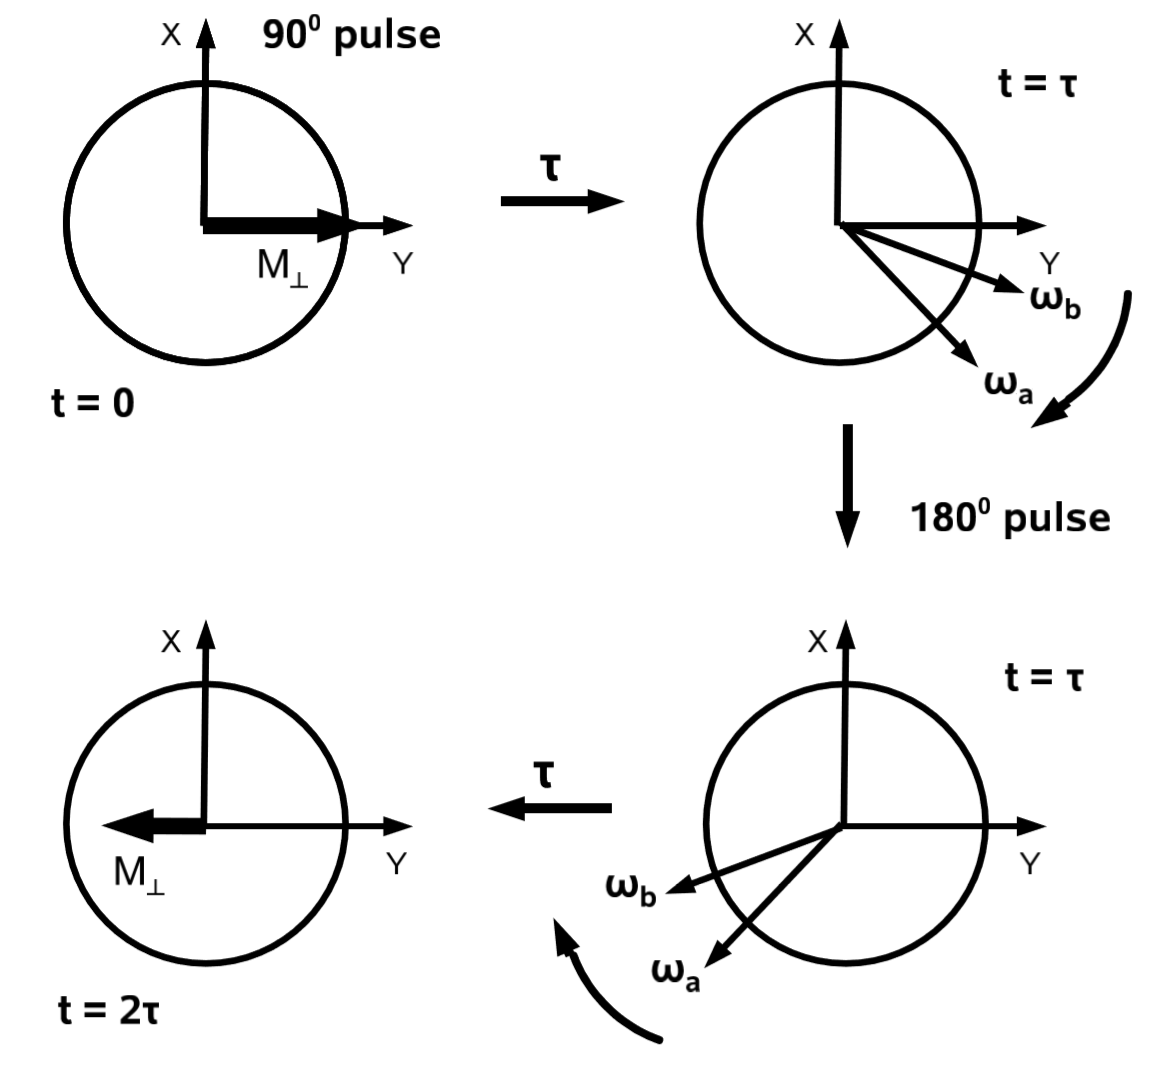
\includegraphics[scale=0.53]{images/spin_echo.png}
	\caption{Dephasing of transverse magnetization $\vec{M_{\perp}}$} taken from \cite{manual}
	\label{spin-spin}
\end{figure} \\
$\omega_a$ and $\omega_b$ are denoting 2 protons which experience different $\omega_L$'s, which is caused by the inhomogeneities of the external $\vec{B_0}$.\\
To measure the loss of amplitude we analyse the Fourier spectrum at the time $t=2\tau$ and integrate over the peak at the $\omega_L$. If we repeat the process for different $\tau$ we will get a curve. This curve should follow \eqref{15}, since the calculated amplitude is proportional to $\vec{M_{\perp}}$, and with the help of a fit we can extract the $T_{2,SE}$.
\vspace{3mm} \\
For the second method, the Carr-Purcell method, we also apply a $90\degree$ pulse at first and apply a $180\degree$ pulse at $t=\tau$. At $t=2\tau$ the system should be in phase, but will dephase shortly after, same as in method one. We then apply another $180\degree$ at $t=3\tau$ which will lead to a fully in phase system at $t=4\tau$ again. This process can be continued for $180\degree$ at odd multiples of $\tau$ to get the system in phase at even $\tau$. This process is a lot more precise for big $\tau$ in comparison to the spin-echo method, which gets inaccurate because of the molecular diffusion (the protons move away from their original position) and inhomogeneities in the field.\\
The measured amplitudes should still follow \eqref{15}.
\subsubsection{Spin-lattice relaxation time $T_{1}$}
Spin-latice relaxation is caused by the interaction between the magnetic dipoles and the external magnetic field $\vec{B_0}$ and contributes to the parallel magnetization. This relaxation process is described by \eqref{13}, which is solved by
\begin{equation}
	\label{16}
	M_{\parallel}(t) = M_{0}(1-2e^{-\frac{t}{T_{1}}}).
\end{equation}
We measure $T_1$ also with the spin-echo method. But this time we start at $t=0$ with a $180\degree$ pulse and follow up after $t=\tau$ with a $90\degree$ pulse. We then measure the amplitude at $t=2\tau$ for different $\tau$ and expect the resulting curve to follow \eqref{16}.
\subsection{Chemical shift}\label{chemShift}
\begin{figure}[h]
	\begin{subfigure}{0.5\textwidth}
	\centering
	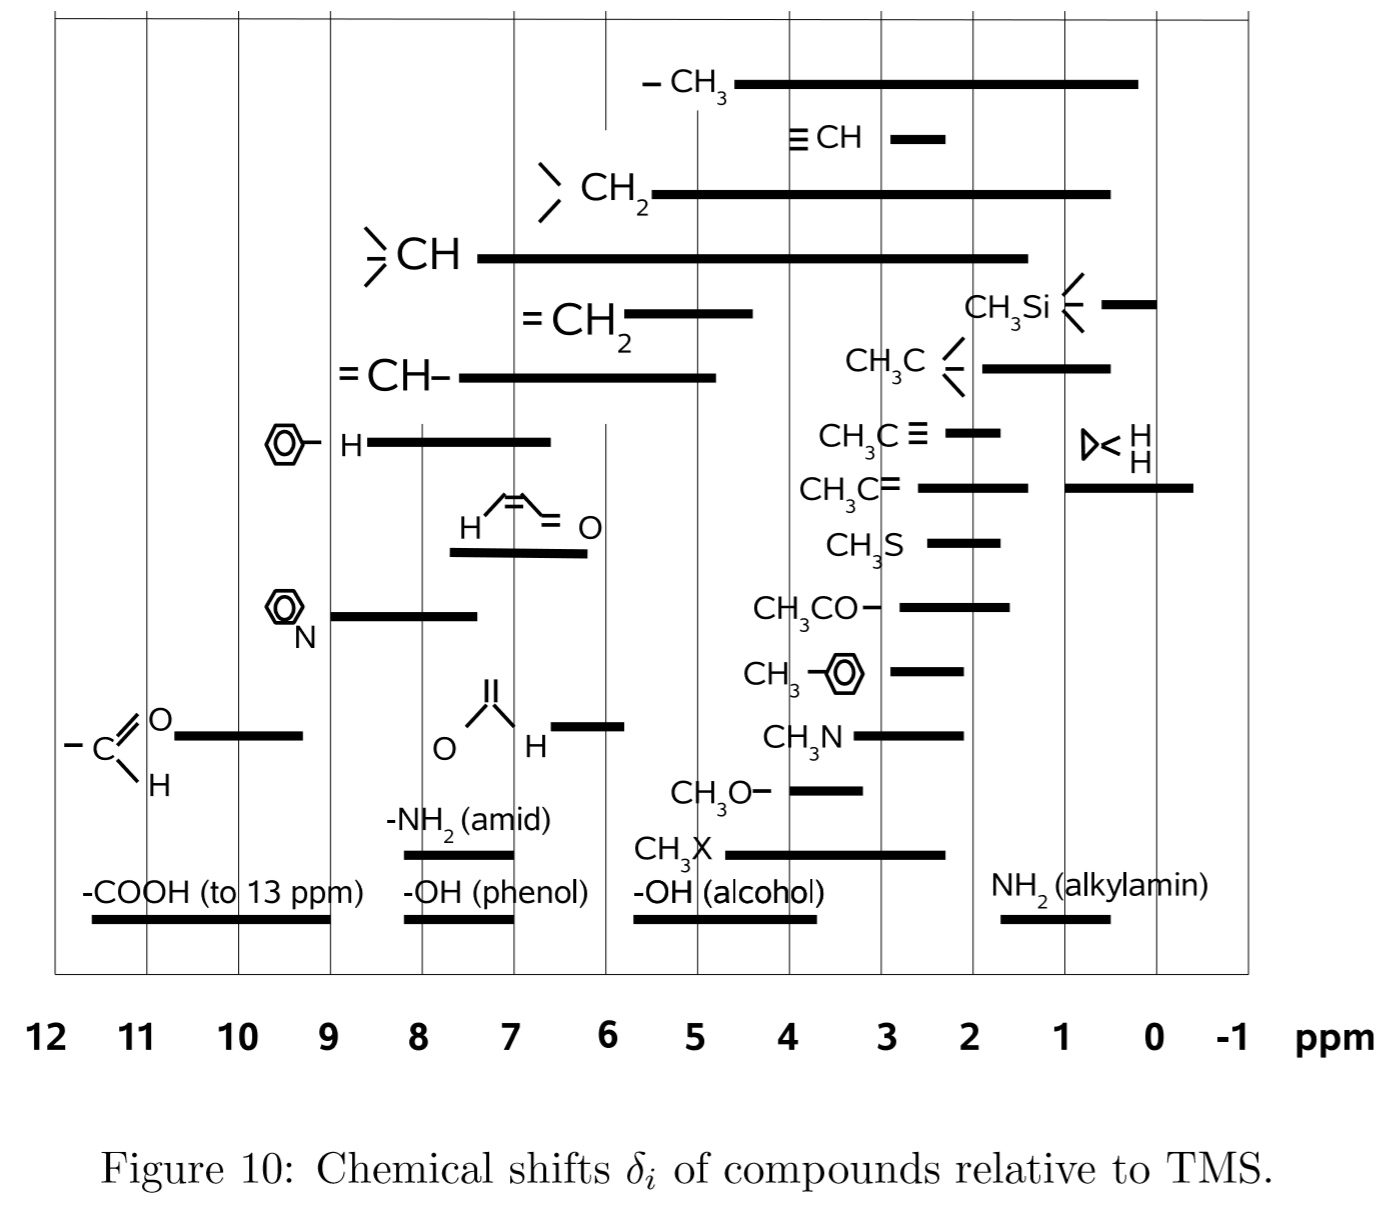
\includegraphics[width=0.7\linewidth ,height=4cm]{images/ChemShift.png}
	\caption{Chemical Shift $\delta_i$}
	\label{shi1}
	\end{subfigure}
	\begin{subfigure}{0.5\textwidth}
	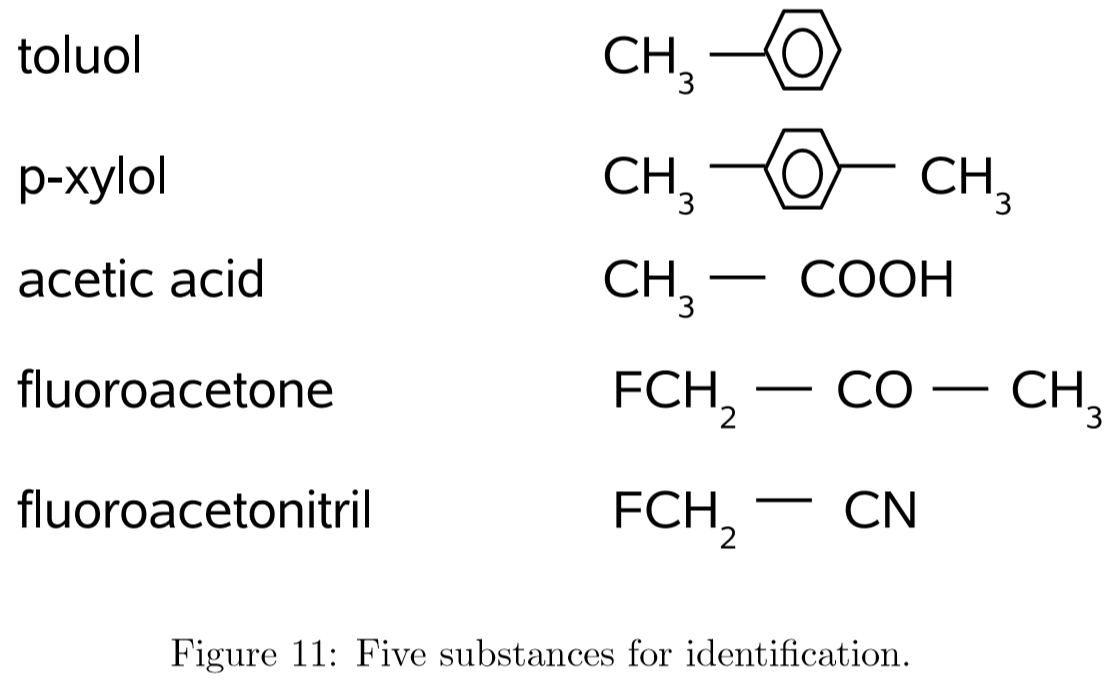
\includegraphics[width=0.7\linewidth ,height=4cm]{images/substances.png}
	\caption{Substances to be sorted}
	\label{shi2}
	\end{subfigure}
	\caption{Chemical Shift taken from \cite{manual}}
	\label{shi3}
\end{figure}
If a proton is bound by a molecule, it will experience a magnetic field that is weaker than the external magnetic field $\vec{B_0}$, since the electrons are shielding parts of it. This leads to a new resonance frequency $\omega_i$ for the proton bound by the molecule. This modified resonance frequency can be used to identify unknown substances. To do so, it is easiest to compare it to a reference substance which you can easily identify in a Fourier spectrum, since the whole frequency scale is dependent on $\vec{B_0}$ which means it's a relative scale and one can't use absolute frequency values. We are using Tetra-Methyl-Silan or TMS since its peak will always be clearly visible and in our case always be the peak on the most left. With the help of $\omega_{TMS}$ one can define a chemical shift
\begin{equation}\label{deltashift}
	\delta_i = \frac{\omega_{TMS}-\omega_{i}}{\omega_{L}}
\end{equation} 
for different molecule parts in reference to TMS as shown above in figure \ref{shi1}. In this experiment we want to identify the substances in figure \ref{shi2} from 5 different probes. \\
\subsection{Imaging with NMR}\label{imagening}
Imaging with NMR is one of the most notable achievements of NMR. By adding a gradient to the external field $\vec{B_0}$ we create a coordinate dependency of the $B_0$ field, which implies a coordinate dependent $\omega_L$. There are two different approaches to determine the density of the NMR-active material of the probe in 1 dimension.
\vspace{2mm}\\
The first method is called frequency coding, where one has a fixed gradient over time and measures the  NMR signal in set times $t_n = n \Delta t$. Then one can do a discrete Fourier transform of the $N$ measurements and gets a finite amount of $M_{\perp}(n \Delta z)$ for the different coordinates. 
\vspace{2mm}\\
The second method is called phase coding, where one has a fixed time and determines the phase of the precession all at the same time $t = t_0$. From that you again get a discrete amount of data points with which you can do a discrete Fourier transform. 
\vspace{2mm}\\
The main difference between these two methods is the time needed to record the data needed. The first method requires $T_f = N \cdot \Delta t$ compared to the $T_{\Phi} = t_0$ for the second method.
\vspace{3mm}\\
For 2 dimensions you have to use a combination of both since you need to determine 2 coordinates with just 1 signal. First a slice gets selected which is used to derive the positional information. Then it does phase coding for a set gradient while measuring the NMR signal over time with a set time distance $t_m$. After finishing the frequency coding it changes the gradient, selects a slice again and does a phase coding again followed by a frequency coding. This process is repeated for $N$ different gradients, taking $M \Delta t$ for each gradient. That leads to $N \times M$ data points which then can be transformed with a 2 dimensional Fourier transform into the image matrix of the object. One of the $N$ cycles is illustrated below \ref{2dfourier}.\\
\begin{figure}[h]
	\centering
	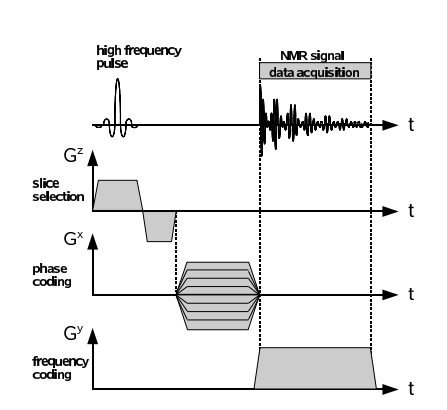
\includegraphics[width=0.63\linewidth ,height=7cm]{images/2d_fourier.png}
	\caption{One of the N Loops needed for 2D Imaging taken from \cite{manual}}
	\label{2dfourier}
\end{figure}